
%(BEGIN_QUESTION)
% Copyright 2006, Tony R. Kuphaldt, released under the Creative Commons Attribution License (v 1.0)
% This means you may do almost anything with this work of mine, so long as you give me proper credit

Calculate the liquid flow rate measured by this V-notch weir, given a crest height ($H$) of 5.5 inches:

$$\includegraphics[width=15.5cm]{i00712x01.eps}$$

$$Q = 2.48 \left( \tan {\theta \over 2} \right) H^{2.5} \hbox{\hskip 20pt V-notch weir}$$

\noindent
Where,

$Q$ = Volumetric flow rate, in cubic feet per second (ft$^{3}$/s)

$\theta$ = V-notch angle, in degrees ($^{o}$)

$H$ = Head, in feet (ft)

\vskip 10pt

Provide an answer for flow rate in units of cubic feet per second (CFS), gallons per minute (GPM), and in millions of cubic feet per day (MCFD), which means millions of cubic feet per 24-hour period):

\vskip 10pt

$Q$ = \underbar{\hskip 50pt} CFS

\vskip 10pt

$Q$ = \underbar{\hskip 50pt} GPM

\vskip 10pt

$Q$ = \underbar{\hskip 50pt} MCFD

\underbar{file i00712}
%(END_QUESTION)





%(BEGIN_ANSWER)

4 points for the correct cubic-feet-per-second (CFS) answer, 3 points for the other two:

\vskip 10pt

$Q$ = \underbar{\bf 0.2822} CFS

\vskip 10pt

$Q$ = \underbar{\bf 126.6} GPM

\vskip 10pt

$Q$ = \underbar{\bf 0.02438} MCFD


%(END_ANSWER)





%(BEGIN_NOTES)

{\bf This question is intended for exams only and not worksheets!}.

%(END_NOTES)


